\chapter{Objetivos del trabajo y herramientas necesarias}

\section{Introducción}
Habiendo tratado en el capítulo anterior el fundamento teórico que concierne a las nubes de puntos, sensores con los que adquirirlas y el procesamiento software de las mismas se procede en este capítulo a explicar con mayor profundidad los módulos de la librería de PCL de interés para el presente trabajo.

Además, se presentan los objetivos que se quieren alcanzar al término del TFG así como las herramientas necesarias para conseguirlo.

\section{Objetivos del TFG}
Una vez establecido el fundamento teórico relativo a las nubes de puntos en general y a la librería PCL se procede a continuación a exponer el motivo de este trabajo fin de grado.

Se tiene un doble objetivo que involucra por una parte la reproducción de algoritmos ya existentes y por otra la optimización de parte de los mismos.
\begin{itemize}
\item[1)] La parte de reproducción de algoritmos existentes se refiere a desarrollar un programa escrito en C++ que sea capaz de extraer keypoints de una nube de puntos cualquiera siempre y cuando su formato sea PCD. Para ello se hace uso de la documentación ofrecida por la web oficial de PCL y los conocimientos propios de programación en C++. 
\item[2)] Habiendo desarrollado dicho programa, se procede a estudiar en detalle las partes de la librería PCL que utiliza, comprender cómo funcionan y medir tiempos de ejecución de los diferentes métodos nativos de PCL involucrados en todo el proceso de extracción de keypoints. De este modo, se detecta el algoritmo de mayor tiempo de ejecución y por lo tanto el de mayor carga computacional. Finalmente, se estudia la mencionada parte del código y se plantea cómo crear hardware digital exclusivamente para la optimización de la parte del código de PCL y no de las librerías adicionales en las que se apoya. Puesto que no todo tipo de software es sintetizable en hardware, deberán hacerse simplificaciones o incluso cambios sustanciales al código original para posibilitar su síntesis.
\end{itemize}


Se tienen a continuación algunas notas importantes sobre el desarrollo del trabajo:
\begin{itemize}
\item[•] Para llevar a cabo el objetivo 2) se utilizarán conocimientos de High Level Synthesis (HLS) que se traduce como síntesis de alto nivel y puede definirse como un proceso automatizado que interpreta una descripción algorítmica de un deseado comportamiento y crea hardware digital que implementa dicho comportamiento. De esta manera se podrá crear una Intellectual Property (IP) que contiene la optimización mencionada y así hacer uso de ella.
\item[•] La plataforma sobre la que se comprobará la compleción de dichos objetivos es una FPGA cuyas características se exponen en el apartado \ref{herraminetas_hardware}
\item[•] Como objetivo o punto adicional, se desarrolla también código en C++ para mostrar nubes de nubes de puntos por pantalla y así poder representar de una manera visual e intuitiva diferentes conjuntos de puntos y las operaciones efectuadas sobre los mismos. Es importante destacar que esta funcionalidad no funciona en la FPGA ya que no tiene interfaz gráfica.

\end{itemize}

 

\section{Descripción de herramientas para desarrollar el trabajo}
Para realizar el presente trabajo se requieren herramientas que pueden clasificarse en dos tipos: software y hardware.

\subsection{Herramientas software}
\subsubsection{Máquina virtual}
Se hace uso de una máquina virtual con Ubuntu\cite{ubuntu} 18.04.1 64 bits ya que es un sistema operativo que facilita la instalación y uso de PCL y otras librerías, no como Windows. 

Por lo tanto, a partir de este punto, salvo que se mencione lo contrario, el sistema de archivos e instrucciones ejecutadas por línea de comandos así como demás características propias de diferentes sistemas operativos se refieren a un sistema operativo basado en Linux.

La máquina virtual se crea haciendo uso del software VirtualBox\cite{virtualbox} el cual facilita la creación y personalización de máquinas virtuales no solamente basadas en Linux sino en cualquier otro sistema operativo.

%https://www.virtualbox.org/

\subsubsection{PCL}
Una vez se dispone de la máquina virtual, es necesario instalar las librerías de PCL\cite{pcl_installation}. Para ello se visita la web oficial de PCL pues ésta ofrece las instrucciones adecuadas. Para poder instalar PCL en linux se deben ejecutar los siguientes comandos:

%http://pointclouds.org/downloads/

\begin{verbatim}
sudo add-apt-repository ppa:v-launchpad-jochen-sprickerhof-de/pcl
sudo apt-get update
sudo apt-get install libpcl-all
\end{verbatim}

La primera instrucción añade al sistema el repositorio en el que se encuentra la librería, el segundo busca actualizaciones disponibles y por último se procede a la instalación de todos los archivos actualizados.

Cuando la instalación está completa, se generan una serie de carpetas en el directorio /usr/include:

\begin{itemize}
\item[•]pcl-1.8: Es la versión 1.8 de la librería de PCL. Contiene en su interior la carpeta pcl que con todos los módulos de PCL estructurados correctamente.
\item[•]eigen3: Librería eigen que se encuentra bajo la carpeta Eigen dentro de este directorio.
\item[•]FLANN: Librería FLANN que se encuentra bajo la carpeta flann dentro de este directorio.
\item[•]vtk-x: versión x de la librería vtk 
\end{itemize}

\subsubsection{Vivado Design Suite HLx Editions}
Ya está instalado PCL en el sistema, ahora falta adquirir una herramienta adecuada para síntesis de software en hardware digital y configuración de FPGAs. Para ello se elige la herramienta vivado HLS de Xilinx. Accediendo a la web oficial de descargas\cite{vivado_descarga} se puede descargar la versión deseada de este software ya sea como un archivo comprimido un instalador web para mayor comodidad. En este caso se elige la versión 2017.1

%https://www.xilinx.com/support/download.html
%https://www.xilinx.com/products/design-tools/vivado/integration/esl-design.html

\subsection{Herramientas hardware} \label{herraminetas_hardware}
La principal herramienta hardware de la que se dispone y sobre la cual se comprobarán los resultados de la aplicación de los objetivos del presente trabajo es una Pynq-Z1\cite{pynq} del modelo xc7z020clg400-1 que se puede ver en la figura \ref{fig:pynq}. Se trata de una FPGA, siglas del inglés ``Field Programmable Gate Array'' y se trata, a grandes rasgos, de un dispositivo que combina recursos hardware y software para aprovechar la potencia de la ejecución en paralelo de tareas del primero y la flexibilidad, rutinas software y tareas relacionadas con sistemas operativos del segundo. Los recursos hardware quedan dentro de lo que se conoce como Programmable Logic (PL) o lógica programable y los recursos software en el Processing System (PS)

Además, una FPGA dispone de dos capas: aplicación y configuración. La primera se compone de todos sus recursos hardware que han de ser configurados e interconectados haciendo uso de la segunda, la capa de configuración en la que se carga un ``bitstream'' es decir un archivo de configuración que se puede generar, entre otras formas, haciendo uso del programa Vivado de Xilinx y que permite para cada ``bitstream'' que se cargue, dotar a la FPGA de diferentes funcionalidades.



\begin{figure}[H]
\centering
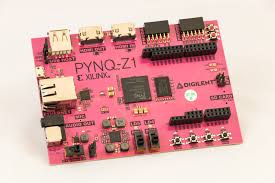
\includegraphics[scale=1.0]{pynq}
  \caption{FPGA Pynq-Z1 xc7z020clg400-1 de Xilinx.}\label{fig:pynq}
\end{figure}

La Pynq-Z1 es el soporte hardware para la tecnología PYNQ que es de libre uso. Ésta permite explotar las capacidades de los sistemas en chip programables sin tener que diseñar circuitos de lógica programable la cual ya ha sido diseñada usando el lenguaje de programación Python. De este modo, los circuitos de lógica programable son importados como librerías hardware y configurados según sus APIs de la misma forma que las librerías software son importadas y configuradas.

Algunas de las características principales de la Pynq-Z1 son:

\begin{itemize}
\item[•] Un procesador Cortex-A9 de dos núcleos a 650MHz
\item[•] Controlador de memoria DDR3 con 8 canales DMA y 4 puertos esclavos AXI3 de alto rendimiento
\item[•] Periféricos con elevado ancho de banda: Ethernet 1G, USB 2.0 y SDIO 
\item[•] Controlador de periféricos de gran ancho de banda: SPI, UART, CAN, I2C
\item[•] 630KB de memoria RAM
\item[•] Programable con JTAG, flash Quad-SPI y tarjeta micro SD
\end{itemize}

\section{Conclusiones}
Con el cierre del presente capítulo terminan las explicaciones fundamentales tanto de teoría como de herramientas que permiten estructurar el TFG.

En el siguiente capítulo se mostrarán las primeras tareas que giran entorno a la librería PCL para así poder visualizar nubes de puntos y extraer keypoints de las mismas.

